\documentclass[10pt,aspectratio=169]{beamer}

\usetheme{metropolis}
\metroset{sectionpage=none}

\usepackage{amsmath,amssymb,amsfonts}
\usepackage{bm}
\usepackage{booktabs}
\usepackage{tikz}
\usepackage{xcolor}
\usepackage{pgfplots}
\pgfplotsset{compat=1.18}
\usetikzlibrary{arrows.meta, positioning, shapes.geometric, fit, backgrounds,
                decorations.pathreplacing, decorations.markings, calc}

% Useful macros
\newcommand{\T}{\mathcal{T}}
\newcommand{\Hh}{\mathcal{H}}
\newcommand{\E}{\mathbb{E}}
\newcommand{\R}{\mathbb{R}}
\newcommand{\N}{\mathcal{N}}
\newcommand{\indep}{\perp\!\!\!\perp}

\title{Causal inference in high-dimensional survival analysis}
\subtitle{A Bayesian regression trees approach}
\date{}
\author{Tijn Jacobs \\
\small joint work with Wessel N.\ van Wieringen and St\'ephanie L.\ van der Pas}
\institute{Vrije Universiteit Amsterdam}

\definecolor{myaccent}{HTML}{0077B3}
\definecolor{horseshoeorange}{HTML}{E5A33D}
\definecolor{partitionred}{HTML}{E15A2D}

\setbeamercolor{alerted text}{fg=myaccent}
\setbeamercolor{progress bar}{fg=myaccent}
\setbeamercolor{frametitle}{bg=myaccent, fg=white}
\setbeamercolor{normal text}{fg=black!90, bg=white}

\usepackage{graphicx}
\usepackage{qrcode}
\titlegraphic{%
  \vspace{6.5cm}%
  \hfill
\includegraphics[height=1cm]{VU-logo-CMYK.pdf}%
}

% Custom blue section divider frame
\newcommand{\sectiondivider}[1]{%
{%
\setbeamercolor{background canvas}{bg=myaccent}
\begin{frame}[plain]
\vfill
\begin{center}
\color{white}\fontsize{32}{38}\selectfont #1
\end{center}
\vfill
\end{frame}
}}

\begin{document}

\maketitle


%---------------------------------------------------------
\begin{frame}{Why causal inference in high dimensions?}
\begin{columns}[T,onlytextwidth]
\begin{column}{0.50\textwidth}
\vspace{0.5cm}
\textbf{Modern applications, e.g.\ genomics:}
\begin{itemize}
  \item Thousands of covariates per subject.
  \item Confounding: covariates can influence both treatment and outcome.
\end{itemize}

\onslide<2->{%
\bigskip

\textbf{Pancreatic cancer (PDAC):}
\begin{itemize}
  \item Among the deadliest cancers; median survival $<\,$6 months.
  \item Molecularly heterogeneous across patients.
\end{itemize}

\bigskip

\alert{Does adjuvant radiotherapy improve survival, and for whom?}
}%
\end{column}
\begin{column}{0.50\textwidth}
\begin{minipage}[c][0.75\textheight][c]{\linewidth}
\centering
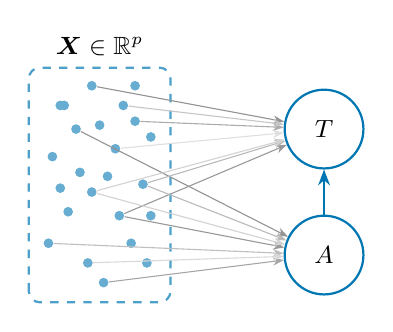
\begin{tikzpicture}[
  baseline=(current bounding box.center),
  xnode/.style={circle, fill=myaccent!60, minimum size=3.5pt, inner sep=0pt},
  bignode/.style={circle, draw=myaccent, thick, minimum size=10mm, font=\small, fill=white},
  arrbase/.style={-{Stealth[length=1.4mm]}, thin}
]
% Cluster of X covariates - deterministic positions
\foreach \i/\x/\y in {
  1/0.15/2.70, 2/0.55/2.95, 3/0.35/2.40, 4/0.05/2.05,
  5/0.75/1.80, 6/0.25/1.35, 7/0.00/0.95, 8/0.50/0.70,
  9/0.90/1.30, 10/1.10/2.50, 11/0.85/2.15, 12/0.20/2.70,
  13/1.20/1.70, 14/0.55/1.60, 15/1.05/0.95, 16/0.15/1.65,
  17/0.70/0.45, 18/1.25/0.70, 19/1.10/2.95, 20/0.65/2.45,
  21/0.40/1.85, 22/0.95/2.70, 23/1.30/2.30, 24/1.30/1.30
}{
  \node[xnode] (X\i) at (\x, \y) {};
}

% Group label
\node[font=\small] at (0.65, 3.45) {$\bm{X} \in \R^p$};

% Dashed border around X cluster
\draw[myaccent!70, dashed, thick, rounded corners=4pt]
  (-0.25, 0.20) rectangle (1.55, 3.18);

% A and T nodes on the right
\node[bignode] (A) at (3.5, 0.80) {$A$};
\node[bignode] (T) at (3.5, 2.40) {$T$};

% Arrows from X to A only (varying tints: dark to light)
\foreach \i/\col in {3/gray!85, 17/gray!70, 7/gray!50, 8/gray!30}{
  \draw[arrbase, \col] (X\i) -- (A);
}

% Arrows from X to T only (varying tints: dark to light)
\foreach \i/\col in {2/gray!85, 10/gray!65, 22/gray!45, 11/gray!25}{
  \draw[arrbase, \col] (X\i) -- (T);
}

% Confounders: arrows from X to BOTH A and T (also varied tints)
\foreach \i/\col in {9/gray!80, 13/gray!55, 14/gray!35}{
  \draw[arrbase, \col] (X\i) -- (A);
  \draw[arrbase, \col] (X\i) -- (T);
}

% A -> T causal arrow
\draw[-{Stealth[length=2mm]}, thick, myaccent] (A) -- (T);

\end{tikzpicture}
\end{minipage}
\end{column}
\end{columns}
\end{frame}

%---------------------------------------------------------
\begin{frame}{Problem setup}
\begin{columns}[T,onlytextwidth]
\begin{column}{0.62\textwidth}
\vspace{0.3cm}
Outcome $T$ is right (or interval) censored.

\bigskip

Covariates $\bm{X} \in \R^p$ are high-dimensional ($p > n$).

\bigskip

Treatment $A \in \{0,1\}$ is not randomised, i.e.\ observational.

\bigskip
\bigskip

\textbf{Research question:}

\smallskip
What is the effect of the treatment on the censored outcome given the covariates (possible confounders)?
\end{column}
\begin{column}{0.38\textwidth}
\centering
\vspace{0.7cm}
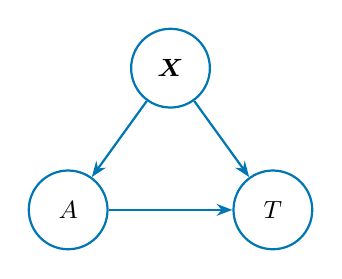
\begin{tikzpicture}[
  every node/.style={circle, draw=myaccent, thick, minimum size=1cm, font=\small},
  arr/.style={-{Stealth[length=2mm]}, thick, myaccent}
]
\node (X) at (0,1.4)     {$\bm{X}$};
\node (A) at (-1.3,-0.4) {$A$};
\node (T) at (1.3,-0.4)  {$T$};
\draw[arr] (X) -- (A);
\draw[arr] (X) -- (T);
\draw[arr] (A) -- (T);
\end{tikzpicture}
\end{column}
\end{columns}
\end{frame}

%---------------------------------------------------------
\begin{frame}{Potential outcomes and causal estimands}
\begin{columns}[T,onlytextwidth]
\begin{column}{0.47\textwidth}
\vspace{0.3cm}
We adopt the potential outcome framework to define causal effects.

\bigskip

For each individual, consider:
\begin{itemize}
  \item $T(1)$: the survival time under treatment.
  \item $T(0)$: the survival time under control.
\end{itemize}

\bigskip

Only one can be observed.
\end{column}
\begin{column}{0.47\textwidth}
\vspace{0.3cm}
\onslide<2->{%
We focus on the \emph{conditional average treatment effect} (CATE):
\bigskip
\[
\tau(x) \;:=\; \E\left[\log T(1) - \log T(0) \mid \bm{X} = x\right],
\]

\bigskip
and the corresponding \emph{acceleration factor} (AF):
\[
\mathrm{AF}(x) \;:=\; \exp\bigl(\tau(x)\bigr).
\]
}
\end{column}
\end{columns}
\end{frame}

%---------------------------------------------------------
\begin{frame}{Acceleration factor: an interpretable estimand}
On the log scale, $\tau(x)$ is a difference. Exponentiated, it becomes a \emph{multiplier on survival time}:
\[
T(1)\,\big|\,\bm{X}=x \;\;\overset{d}{=}\;\; e^{\tau(x)} \cdot T(0)\,\big|\,\bm{X}=x.
\]

\begin{columns}[T,onlytextwidth]
\begin{column}{0.5\textwidth}
\vspace{0.3cm}
\textbf{Acceleration factor} $e^{\tau(x)}$:
\begin{itemize}
  \item Treatment stretches the patient's clock.
  \item $e^{\tau(x)} = 2 \;\Rightarrow\;$ median survival doubles.
  \item Same shape, different time scale.
\end{itemize}
\end{column}
\begin{column}{0.5\textwidth}
\centering
\vspace{0.2cm}
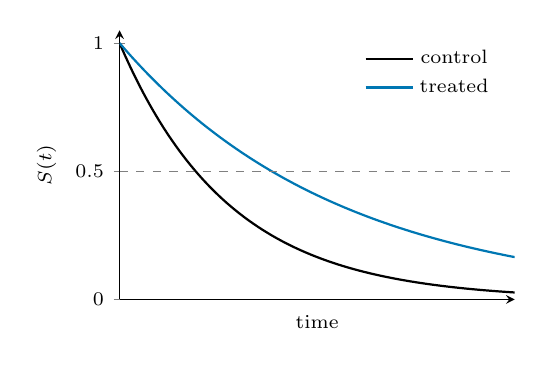
\begin{tikzpicture}
\begin{axis}[
  width=6.6cm, height=5cm,
  xlabel={time}, ylabel={$S(t)$},
  xmin=0, xmax=12, ymin=0, ymax=1.05,
  xtick=\empty, ytick={0,0.5,1},
  legend pos=north east,
  legend style={font=\scriptsize, draw=none},
  axis lines=left,
  tick label style={font=\scriptsize},
  label style={font=\scriptsize},
]
\addplot[domain=0:12, samples=200, thick, black]    {exp(-0.30*x)};
\addlegendentry{control}
\addplot[domain=0:12, samples=200, thick, myaccent] {exp(-0.15*x)};
\addlegendentry{treated}
\draw[dashed, gray] (axis cs:0,0.5) -- (axis cs:12,0.5);
\end{axis}
\end{tikzpicture}
\end{column}
\end{columns}
\end{frame}

%---------------------------------------------------------
\begin{frame}{Why AFT?}

\textbf{1.~Interpretability.}\\
The acceleration factor $e^{\tau(x)}$ acts on the \emph{time scale}, not on hazards.

\bigskip

\textbf{2.~Collapsibility.}\\
The marginal effect is the average of the conditional effects.

\bigskip

\textbf{3.~Robustness.}\\
AFT is robust to omitted independent covariates (Hougaard, 1999).

\vfill

\hfill{\footnotesize\color{myaccent}See Brathovde, Putter, Valberg, Post (2024).}
\end{frame}

%---------------------------------------------------------
\begin{frame}{Identification assumptions}
Potential-outcomes framework $\bigl(T(a), C(a)\bigr)$. Identification proceeds in two steps.

\bigskip

\textbf{1. Causal assumptions} --- link potential outcomes to observables:
\begin{itemize}
  \item \textit{SUTVA}: no interference, well-defined potential outcomes.
  \item \textit{Unconfoundedness}: $T(a) \indep A \mid X$.
  \item \textit{Positivity}: $0 < e(x) := P(A{=}1 \mid X{=}x) < 1$.
\end{itemize}


\vspace{0.6cm}
\textbf{2. Censoring assumption} --- makes the distribution of $T \mid X, A$ identifiable from the censored data $(Y,\delta)$:
\begin{itemize}
  \item \textit{Independent censoring}: $C(a) \indep T(a) \mid X, A$.
\end{itemize}


\end{frame}

%---------------------------------------------------------
\begin{frame}{Unconfoundedness, intuitively}
\begin{columns}[T,onlytextwidth]
\begin{column}{0.55\textwidth}
\vspace{0.3cm}
\textbf{The worry:} sicker patients may be more (or less) likely to be treated $\Rightarrow$ naive comparison mixes treatment effect with baseline differences.

\bigskip

\textbf{Unconfoundedness:}
\[
T(a) \;\indep\; A \;\big|\; \bm{X}, \qquad a \in \{0,1\}.
\]
\emph{Within each $\bm{X}$, treatment looks as if randomised.}

\bigskip

\alert{Match like-for-like:} same $\bm{X}$ $\Rightarrow$ treatment is the only systematic difference.
\end{column}
\begin{column}{0.40\textwidth}
\centering
\vspace{0.5cm}
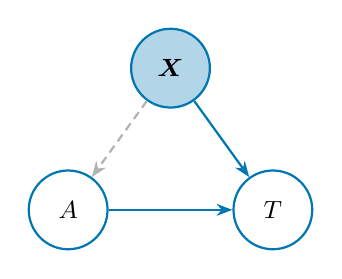
\begin{tikzpicture}[
  every node/.style={circle, draw=myaccent, thick, minimum size=1cm, font=\small},
  arr/.style={-{Stealth[length=2mm]}, thick, myaccent}
]
\node[fill=myaccent!30] (X) at (0,1.4)    {$\bm{X}$};
\node (A) at (-1.3,-0.4) {$A$};
\node (T) at (1.3,-0.4)  {$T$};
\draw[arr, gray!60, densely dashed] (X) -- (A);
\draw[arr] (X) -- (T);
\draw[arr] (A) -- (T);
\end{tikzpicture}

\bigskip
{\footnotesize Conditioning on $\bm{X}$ cuts the dashed back-door arrow.}
\end{column}
\end{columns}
\end{frame}

%---------------------------------------------------------
\begin{frame}{What if we miss a confounder?}
\begin{columns}[T,onlytextwidth]
\begin{column}{0.55\textwidth}
\vspace{0.3cm}
Adjusting for $\bm{X}$ but missing an unmeasured confounder $U$:

\bigskip

\begin{itemize}
  \item Back-door path $A \leftarrow U \rightarrow T$ stays open.
  \item Comparison still picks up the $U$ effect.
  \item \alert{Bias remains --- even with infinite data.}
\end{itemize}

\bigskip

\textbf{High-dimensional consequence:} dropping covariates is risky --- a dropped variable may be a confounder.

\bigskip

\alert{Strategy: keep every covariate in the model.}
\end{column}
\begin{column}{0.40\textwidth}
\centering
\vspace{0.5cm}
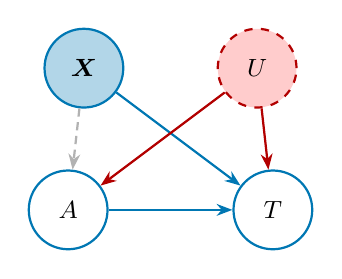
\begin{tikzpicture}[
  every node/.style={circle, draw=myaccent, thick, minimum size=1cm, font=\small},
  arr/.style={-{Stealth[length=2mm]}, thick, myaccent}
]
\node[fill=myaccent!30] (X) at (-1.1,1.4)  {$\bm{X}$};
\node[draw=red!70!black, fill=red!20, dashed] (U) at (1.1,1.4)   {$U$};
\node (A) at (-1.3,-0.4) {$A$};
\node (T) at (1.3,-0.4)  {$T$};
\draw[arr, gray!60, densely dashed] (X) -- (A);
\draw[arr] (X) -- (T);
\draw[-{Stealth[length=2mm]}, thick, red!70!black] (U) -- (A);
\draw[-{Stealth[length=2mm]}, thick, red!70!black] (U) -- (T);
\draw[arr] (A) -- (T);
\end{tikzpicture}

\bigskip
{\footnotesize Unmeasured $U$ leaves an open back-door path $A \leftarrow U \rightarrow T$.}
\end{column}
\end{columns}
\end{frame}

%=========================================================
\sectiondivider{The model}
%=========================================================

%---------------------------------------------------------
\begin{frame}{An accelerated failure time decomposition}
We model the log event-times:
\[
\log T(a) \;=\; f\bigl(x, \hat e(x)\bigr) \;+\; a \cdot \tau(x) \;+\; \varepsilon,
\qquad \varepsilon \sim \N(0, \sigma^2).
\]

\smallskip

\begin{itemize}
  \item $f$:\, prognostic function.
  \item $\hat e(x)$:\, estimated propensity score.
  \item $\tau(x)$:\, heterogeneous treatment effect (CATE).
\end{itemize}

\bigskip

\textbf{Plan.} Place a flexible Bayesian tree-ensemble prior on $f$ and $\tau$, separately.
\end{frame}

%---------------------------------------------------------
\begin{frame}{BART in one slide}
\begin{center}
\begin{minipage}[c]{0.40\linewidth}
  \centering
  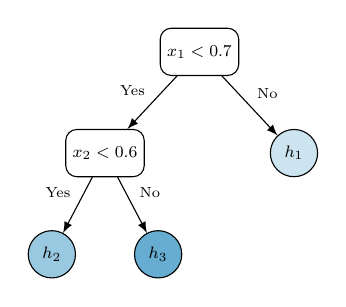
\begin{tikzpicture}[
        scale=0.75, transform shape,
        box/.style={rectangle, draw, rounded corners, align=center,
                    minimum height=8mm, minimum width=13mm, font=\footnotesize},
        leaf/.style={circle, draw, align=center, minimum size=8mm, font=\footnotesize},
        line/.style={-latex}
    ]
    \node [box] (root) {$x_1 < 0.7$};
    \node [box, below=0.9cm of root, xshift=-1.6cm] (left) {$x_2 < 0.6$};
    \node [leaf, fill=myaccent!20, below=0.9cm of root, xshift=1.6cm] (h1) {$h_1$};
    \node [leaf, fill=myaccent!40, below=0.9cm of left, xshift=-0.9cm] (h2) {$h_2$};
    \node [leaf, fill=myaccent!60, below=0.9cm of left, xshift=0.9cm] (h3) {$h_3$};
    \draw[line] (root) -- (left) node[midway, above left,  font=\scriptsize] {Yes};
    \draw[line] (root) -- (h1)   node[midway, above right, font=\scriptsize] {No};
    \draw[line] (left) -- (h2)   node[midway, above left,  font=\scriptsize] {Yes};
    \draw[line] (left) -- (h3)   node[midway, above right, font=\scriptsize] {No};
  \end{tikzpicture}
\end{minipage}\hfill
\begin{minipage}[c]{0.08\linewidth}
  \centering
  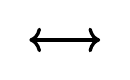
\begin{tikzpicture}
    \draw[<->, very thick] (0,0) -- (0.9,0);
  \end{tikzpicture}
\end{minipage}\hfill
\begin{minipage}[c]{0.40\linewidth}
  \centering
  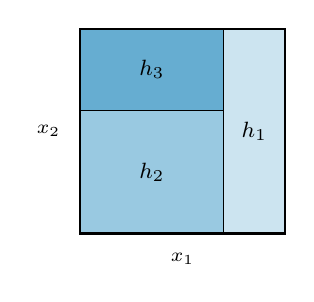
\begin{tikzpicture}[scale=2.6]
    \fill[myaccent!20] (0.7, 0) rectangle (1, 1);
    \fill[myaccent!40] (0, 0)   rectangle (0.7, 0.6);
    \fill[myaccent!60] (0, 0.6) rectangle (0.7, 1);
    \draw[thick] (0, 0) rectangle (1, 1);
    \draw[thin] (0.7, 0) -- (0.7, 1);
    \draw[thin] (0, 0.6) -- (0.7, 0.6);
    \node[below, font=\scriptsize] at (0.5, -0.05) {$x_1$};
    \node[left,  font=\scriptsize] at (-0.05, 0.5) {$x_2$};
    \node[font=\footnotesize] at (0.85, 0.5) {$h_1$};
    \node[font=\footnotesize] at (0.35, 0.3) {$h_2$};
    \node[font=\footnotesize] at (0.35, 0.8) {$h_3$};
  \end{tikzpicture}
\end{minipage}
\end{center}

\vspace{0.2cm}

\textbf{Model.} $g(x) = \sum_{j=1}^{m} g(x;\, \T_j, \Hh_j)$ --- a sum of many shallow trees, each piecewise constant on a partition of the covariate space.

\vspace{0.3cm}

\textbf{Prior.}
\begin{itemize}
  \item Tree shape $\T_j$: depth-penalised Galton--Watson.
  \item Step heights $\Hh_j$: i.i.d.\ Gaussian, variance $\propto 1/m$.
\end{itemize}
\end{frame}

%---------------------------------------------------------
\begin{frame}{Where could you regularise a tree ensemble?}
Two places to regularise:

\bigskip

\begin{enumerate}
  \item \textbf{Via the tree structure} $\T_j$ --- depth penalty, splitting rules, covariate selection (DART, Soft-BART, \ldots).
  \bigskip
  \item \textbf{Via the step heights} $\Hh_j$ --- shrink the \emph{magnitudes} of step heights.
\end{enumerate}

\bigskip

Existing work focuses on (1), but in high dimensions controlling the tree structure either fails to shrink enough or drops relevant confounders.

\bigskip

\alert{Our proposal: regularise through (2) --- a global--local shrinkage prior on the step heights.}
\end{frame}

%---------------------------------------------------------
\begin{frame}{Connection to the normal means model}
\begin{columns}[T,onlytextwidth]
\begin{column}{0.5\textwidth}
\vspace{0.3cm}
The normal means model:
\[
Y_i = \theta_i + \varepsilon_i,
\qquad \varepsilon_i \sim \N(0, \sigma^2).
\]

\bigskip

When the partition becomes fine, each step height effectively fits a single observation.

\bigskip

\alert{Natural place to plug in a global--local shrinkage prior.}
\end{column}
\begin{column}{0.5\textwidth}
\centering
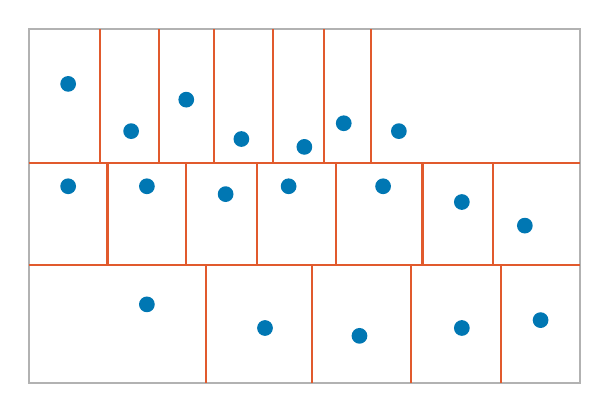
\begin{tikzpicture}[scale=1.0]
\draw[gray!60, thick] (0, 0) rectangle (7, 4.5);
\foreach \x/\y in {
  0.5/3.8, 2.0/3.6, 1.3/3.2, 2.7/3.1, 3.5/3.0,
  4.0/3.3, 4.7/3.2, 0.5/2.5, 1.5/2.5, 2.5/2.4,
  3.3/2.5, 4.5/2.5, 5.5/2.3, 6.3/2.0, 1.5/1.0,
  3.0/0.7, 4.2/0.6, 5.5/0.7, 6.5/0.8
}{
  \fill[myaccent] (\x, \y) circle (0.10);
}
\draw[partitionred, thick] (0, 1.5) -- (7, 1.5);
\draw[partitionred, thick] (0, 2.8) -- (7, 2.8);
\foreach \x in {0.9, 1.65, 2.35, 3.1, 3.75, 4.35}{
  \draw[partitionred, thick] (\x, 2.8) -- (\x, 4.5);
}
\foreach \x in {1.0, 2.0, 2.9, 3.9, 5.0, 5.9}{
  \draw[partitionred, thick] (\x, 1.5) -- (\x, 2.8);
}
\foreach \x in {2.25, 3.6, 4.85, 6.0}{
  \draw[partitionred, thick] (\x, 0) -- (\x, 1.5);
}
\end{tikzpicture}
\end{column}
\end{columns}
\end{frame}

%---------------------------------------------------------
\begin{frame}{Horseshoe prior on the step heights}
\begin{columns}[T,onlytextwidth]
\begin{column}{0.60\textwidth}
\vspace{0.2cm}
For a tree $\T$ with leaves $\ell = 1, \ldots, L$:
\[
h_\ell \mid \lambda_\ell^2, \gamma^2 \;\sim\; \N\bigl(0,\, \lambda_\ell^2\, \gamma^2\bigr),
\]
\[
\lambda_\ell \sim \mathcal{C}^+(0,1), \quad \gamma \sim \mathcal{C}^+(0,1).
\]

\bigskip

\textbf{Two defining features:}
\begin{itemize}
  \item \alert{Pole at zero} --- strong shrinkage of noise.
  \item \alert{Heavy tails} --- large signals are not shrunk.
\end{itemize}

\bigskip

\textbf{Global--local:} $\gamma$ pulls everything to zero; $\lambda_\ell$ lets individual leaves escape.\\
\end{column}
\begin{column}{0.40\textwidth}
\centering
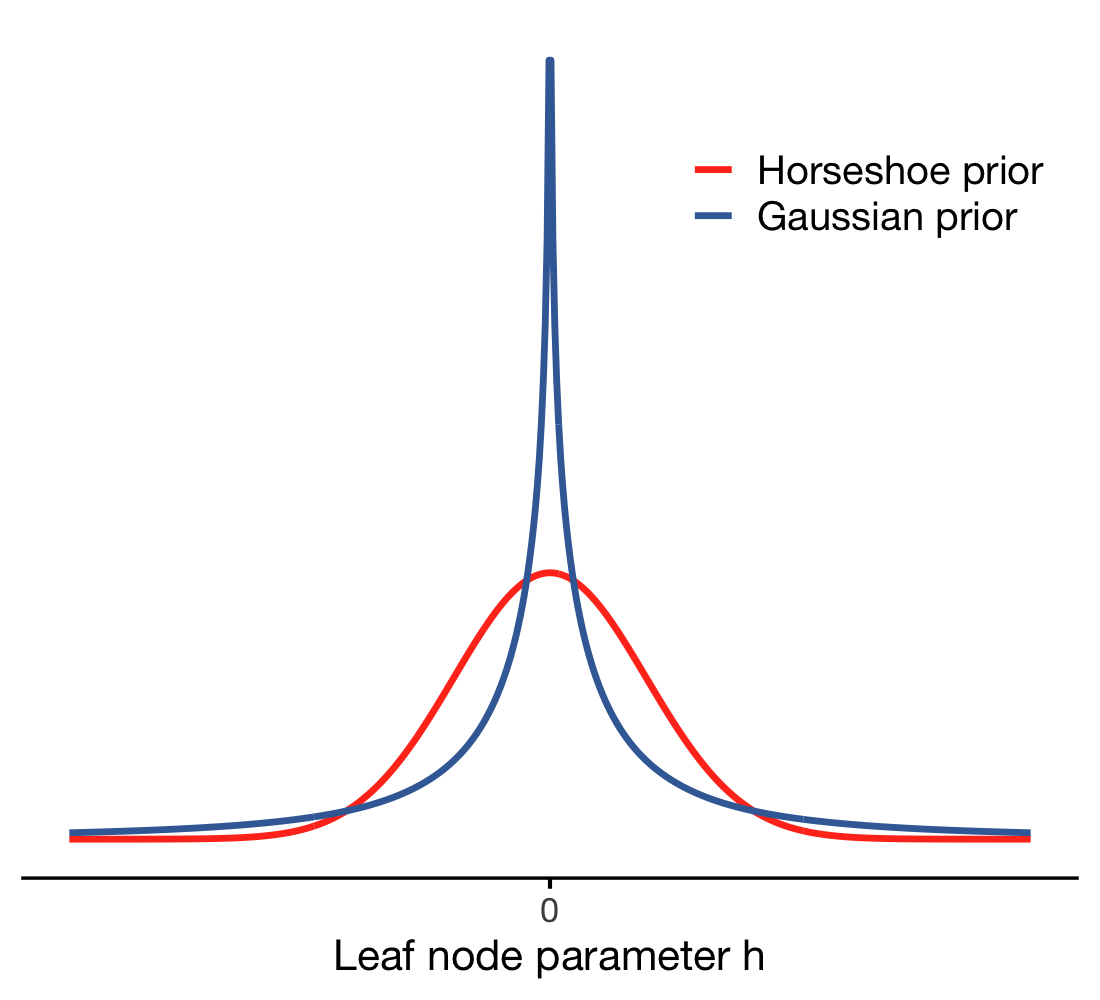
\includegraphics[width=\linewidth]{Horseshoe_plot_ICSDS.png}
\end{column}
\end{columns}
\end{frame}

\begin{frame}{Horseshoe prior on the step heights}
Reparametrise:  $\kappa_\ell = 1 / (1 + \lambda_\ell^2 \gamma^2) \in [0,1]$. Then the posterior mean is
\[
\widehat\theta \;=\; (1 - \kappa_\ell)\,\bar y.
\]

\bigskip

\begin{columns}[T,onlytextwidth]
\begin{column}{0.45\textwidth}
\vspace{0.4cm}
\textbf{Under the horseshoe prior:}
\[
\kappa_\ell \;\sim\; \mathrm{Beta}\!\left(\tfrac{1}{2}, \tfrac{1}{2}\right).
\]

\bigskip

\textbf{This density is U-shaped.} It puts mass at the two extremes:
\begin{itemize}
  \item $\kappa_\ell \approx 1$: noise.
  \item $\kappa_\ell \approx 0$: signal.
\end{itemize}

\end{column}
\begin{column}{0.45\textwidth}
\centering
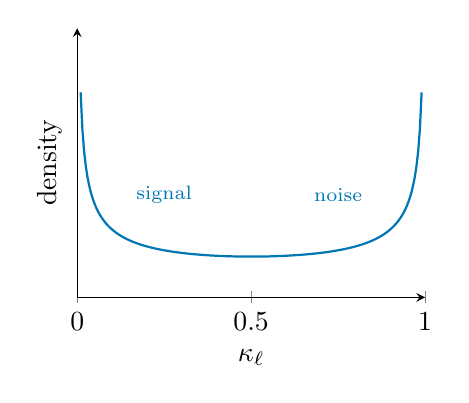
\begin{tikzpicture}
\begin{axis}[
  width=6cm, height=5cm,
  xlabel={$\kappa_\ell$}, ylabel={density},
  xmin=0, xmax=1, ymin=0, ymax=4.2,
  ytick=\empty,
  xtick={0,0.5,1},
  axis lines=left,
]
\addplot[domain=0.01:0.99, samples=200, thick, myaccent]
  {1 / (3.14159 * sqrt(x*(1-x)))};
\node[font=\scriptsize, text=myaccent] at (axis cs: 0.25, 1.6) {signal};
\node[font=\scriptsize, text=myaccent] at (axis cs: 0.75, 1.6) {noise};
\end{axis}
\end{tikzpicture}
\end{column}
\end{columns}
\end{frame}

%---------------------------------------------------------
\begin{frame}{Why horseshoe beats DART}
\textbf{DART} (Linero, 2018): places a Dirichlet prior on the \emph{splitting probabilities} of the covariates.

\bigskip

\begin{columns}[T,onlytextwidth]
\begin{column}{0.32\textwidth}
  Many covariates receive near-zero posterior inclusion probability.

  \bigskip

  Dropping a (weak) confounder $\Rightarrow$ \alert{regularisation-induced confounding}.
\end{column}
\begin{column}{0.60\textwidth}
\centering
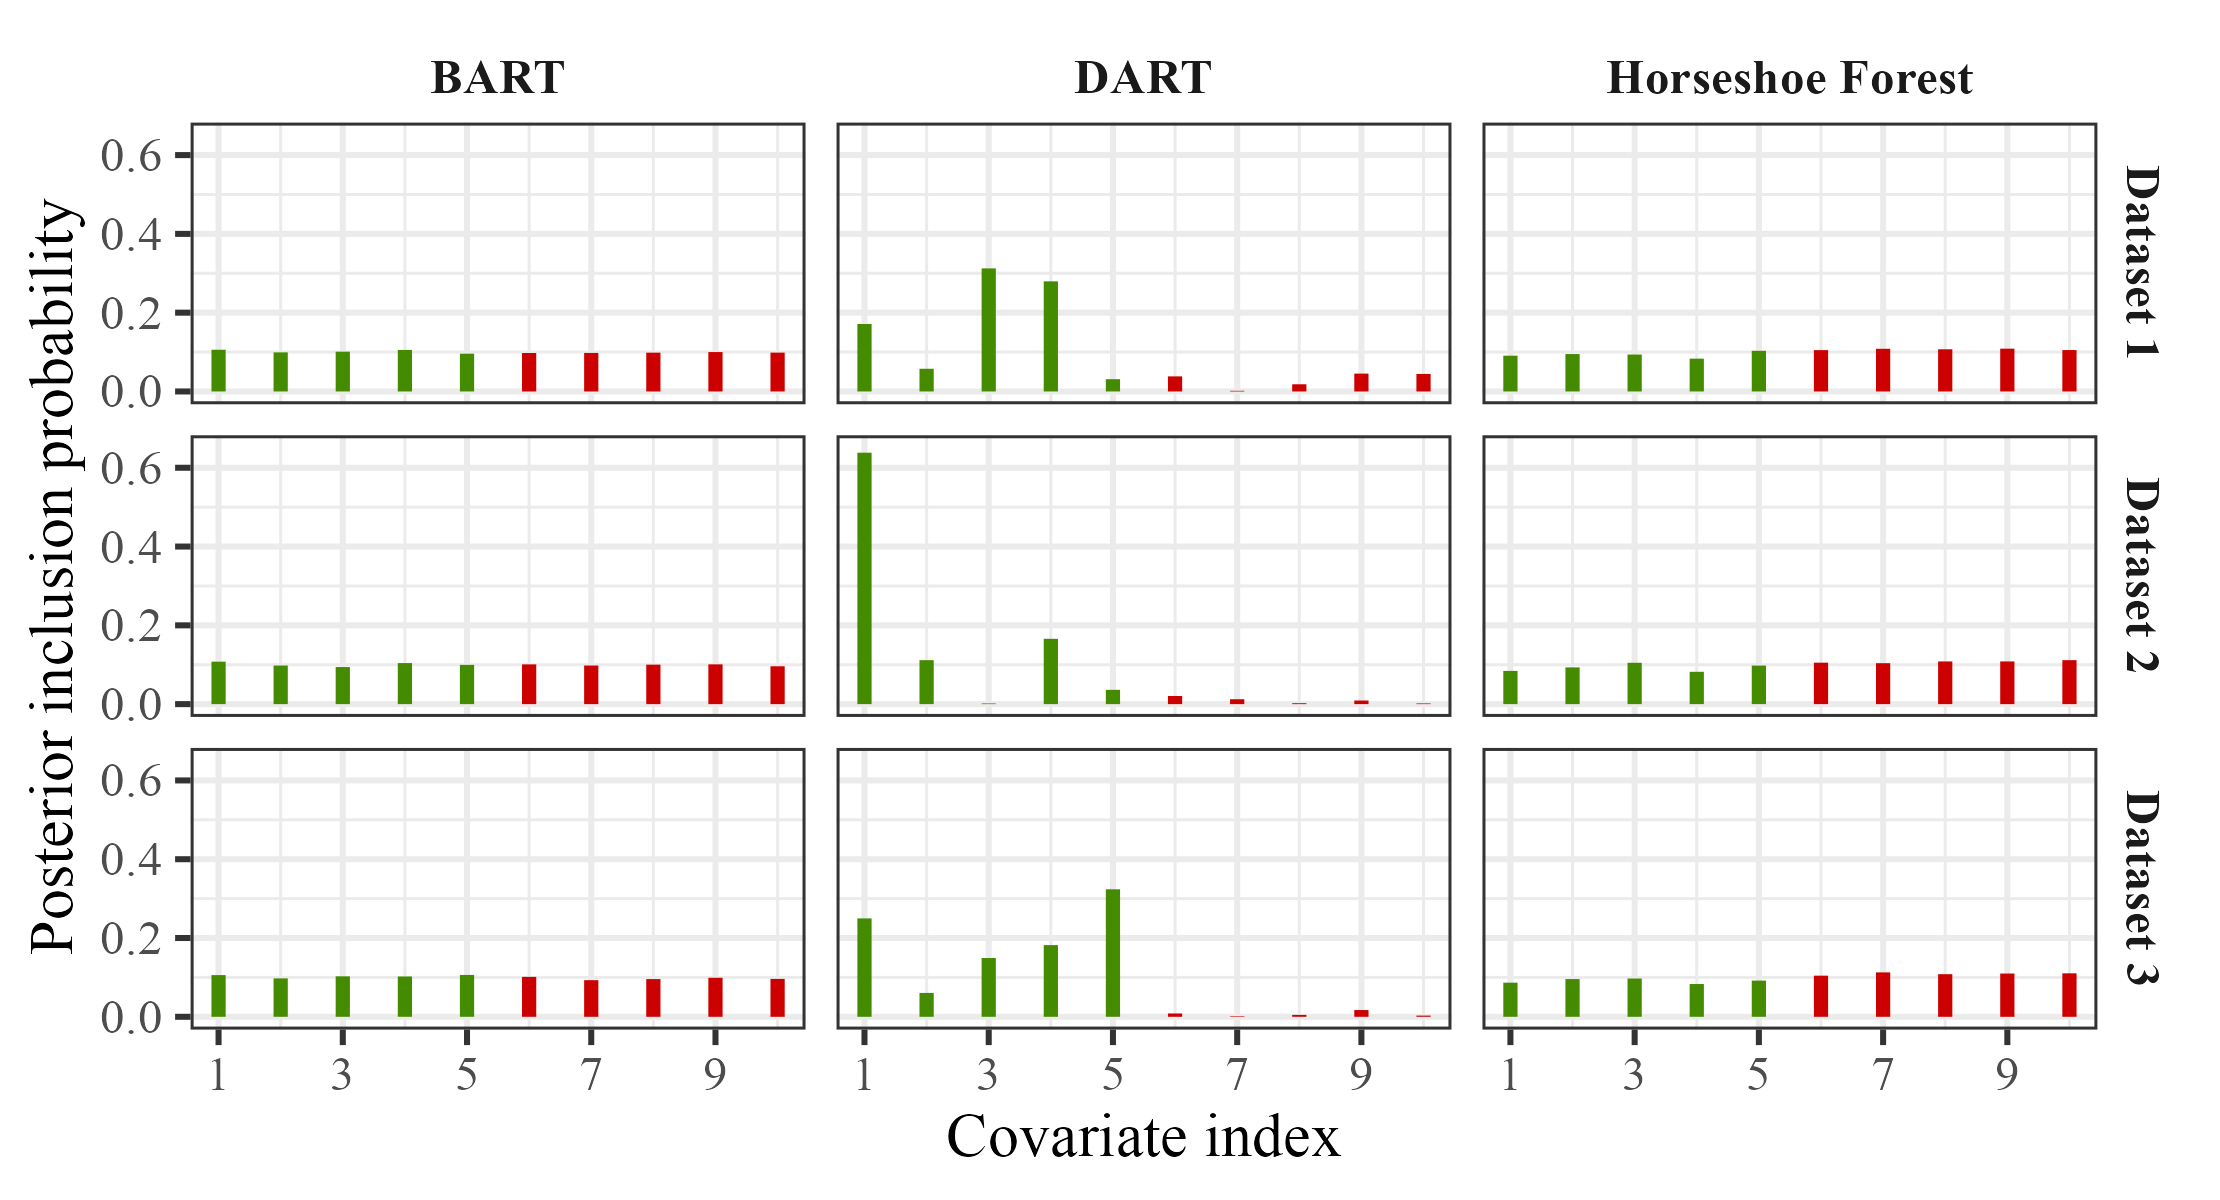
\includegraphics[width=\linewidth]{revision_posterior_inclusion_plot.png}\\
{\footnotesize Posterior inclusion probabilities across covariates.}
\end{column}
\end{columns}

\bigskip

\alert{Horseshoe forest: keep every covariate split-eligible; shrink the \emph{magnitudes} instead.}
\end{frame}

%=========================================================
\sectiondivider{Posterior inference*}
%=========================================================

%---------------------------------------------------------
\begin{frame}{Sampling from the posterior}
Recall the causal model:
\[
\log T(a) \;=\; f(x, \hat e) \;+\; a \cdot \tau(x) \;+\; \varepsilon,
\qquad \varepsilon \sim \N(0, \sigma^2).
\]

\bigskip

The sampling procedure is at the outer level a Gibbs sampler:
\begin{enumerate}
  \item update $f$
  \item update $\tau$
  \item augment censored observations
  \item update $\sigma^2$
\end{enumerate}
\end{frame}

%---------------------------------------------------------
\begin{frame}{Reversible-jump within Gibbs}
\begin{columns}[c,onlytextwidth]
\begin{column}{0.40\textwidth}
The horseshoe prior is \emph{not} Gaussian-conjugate $\Rightarrow$ step heights cannot be marginalised out.

\bigskip

GROW and PRUNE moves change the dimension of $\Hh_j$. We use a \alert{reversible-jump} step with a tailored proposal for $(\T_j, \Hh_j)$.

\end{column}
\begin{column}{0.58\textwidth}
\centering
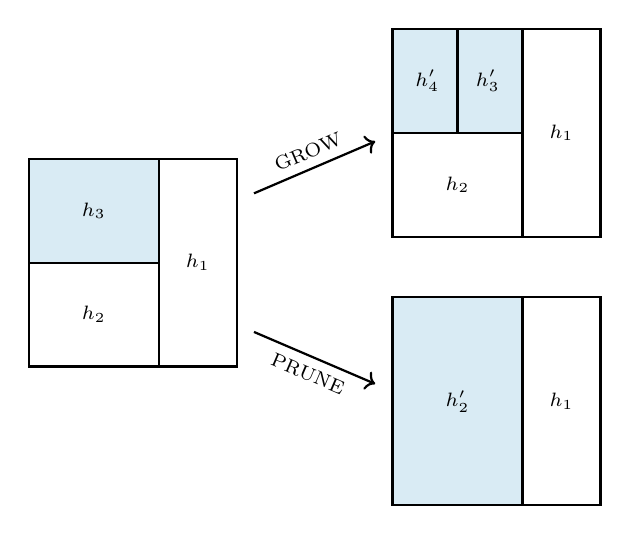
\begin{tikzpicture}[
  scale=1.1, every node/.style={font=\scriptsize}
]
% Parent partition
\fill[myaccent!15] (0,1.2) rectangle (1.5,2.4);
\draw[thick] (0,0) rectangle (2.4,2.4);
\draw[thick] (1.5,0) -- (1.5,2.4);
\draw[thick] (0,1.2) -- (1.5,1.2);
\node at (0.75,1.8) {$h_3$};
\node at (0.75,0.6) {$h_2$};
\node at (1.95,1.2) {$h_1$};

\draw[->, thick] (2.6,2.0) -- (4.0,2.6) node[midway, above, sloped] {GROW};
\draw[->, thick] (2.6,0.4) -- (4.0,-0.2) node[midway, below, sloped] {PRUNE};

% GROW result
\begin{scope}[shift={(4.2,1.5)}]
\fill[myaccent!15] (0,1.2) rectangle (1.5,2.4);
\draw[thick] (0,0) rectangle (2.4,2.4);
\draw[thick] (1.5,0) -- (1.5,2.4);
\draw[thick] (0,1.2) -- (1.5,1.2);
\draw[thick] (0.75,1.2) -- (0.75,2.4);
\node at (0.4,1.8) {$h'_4$};
\node at (1.1,1.8) {$h'_3$};
\node at (0.75,0.6) {$h_2$};
\node at (1.95,1.2) {$h_1$};
\end{scope}

% PRUNE result
\begin{scope}[shift={(4.2,-1.6)}]
\fill[myaccent!15] (0,0) rectangle (1.5,2.4);
\draw[thick] (0,0) rectangle (2.4,2.4);
\draw[thick] (1.5,0) -- (1.5,2.4);
\node at (0.75,1.2) {$h'_2$};
\node at (1.95,1.2) {$h_1$};
\end{scope}
\end{tikzpicture}
\end{column}
\end{columns}
\end{frame}

%---------------------------------------------------------
\begin{frame}{Augmentation of the censored data}
\begin{columns}[T,onlytextwidth]
\begin{column}{0.45\textwidth}
\vspace{0.2cm}
Tanner \& Wong (1987): treat censored event times as latent variables in the Gibbs sampler.

\bigskip

At each iteration $t$, draw the unobserved $\log T_i^{(t)}$ from
\[
\N\!\bigl(\mu_i^{(t)},\, \sigma^{2,(t)}\bigr)
\]
truncated to $(\log Y_i, \infty)$, with
\[
\mu_i^{(t)} = f^{(t)}\!\bigl(x_i, \hat e(x_i)\bigr) + a_i\, \tau^{(t)}(x_i).
\]
\end{column}
\begin{column}{0.50\textwidth}
\centering
\begin{tikzpicture}[scale=0.95]
% T=0 vertical axis (left edge)
\draw[gray!70] (0, -0.3) -- (0, 4.0);
\node[font=\scriptsize, gray] at (0.0, 4.3) {$T = 0$};

% Lifeline 1: Observed event
\draw[->, gray!70, >=stealth] (0, 3.5) -- (5.5, 3.5);
\node[font=\large, gray!80] at (5.5, 3.5) {$\ast$};

% Lifeline 2: Right censored
\draw[->, gray!70, >=stealth] (0, 1.9) -- (3.0, 1.9);
\draw[dotted, gray!70] (3.0, 1.9) -- (7, 1.9);

% Lifeline 3: Interval censored
\draw[->, gray!70, >=stealth] (0, 0.3) -- (3.0, 0.3);
\draw[dotted, gray!70] (3.0, 0.3) -- (5.5, 0.3);
\node[font=\small, gray!80] at (5.55, 0.3) {$\triangleleft$};

% --- Slide 2 onwards: density curve on middle lifeline ---
\onslide<2->{
\draw[myaccent, thick, domain=2.6:6.6, smooth, samples=80, variable=\x]
  plot ({\x}, {1.9 + 1.0*exp(-(\x-4.0)*(\x-4.0)/1.0)});
\node[font=\large, myaccent] at (4.5, 1.9) {$\ast$};
}

% --- Slide 3 onwards: red star and dotted line on middle ---
\onslide<3->{
\node[font=\large, partitionred] at (3.85, 1.9) {$\ast$};
\draw[partitionred, dotted, thick] (3.85, 1.9) -- (3.85, 2.83);
}

% --- Slide 4 onwards: density curve on bottom lifeline ---
\onslide<4->{
\draw[myaccent, thick, domain=3.3:5.3, smooth, samples=80, variable=\x]
  plot ({\x}, {0.3 + 0.55*exp(-(\x-4.3)*(\x-4.3)/0.45)});
\node[font=\large, myaccent] at (4.5, 0.3) {$\ast$};
}

% --- Slide 5 onwards: red star and dotted line on bottom ---
\onslide<5->{
\node[font=\large, partitionred] at (3.95, 0.3) {$\ast$};
\draw[partitionred, dotted, thick] (3.95, 0.3) -- (3.95, 0.78);
}
\end{tikzpicture}
\end{column}
\end{columns}
\end{frame}

%=========================================================
\sectiondivider{Does it work?}
%=========================================================

%---------------------------------------------------------
\begin{frame}{Simulation 1: CATE estimation as $p$ grows}
\textbf{Setting:} $n = 200$, $50 \leq p \leq 5000$, censoring $\approx 35\%$.

\bigskip

\textbf{Data generating process:}
\[
X_i \sim \mathcal{U}[0,1]^p, \quad A_i \sim \mathrm{Ber}(e(x_i)), \quad \log T_i \sim \N\!\bigl(f(x_i) + A_i\, \tau(x_i),\, \sigma^2\bigr),
\]
where $\sigma$ is chosen s.t. $\mathrm{Var}(\log T)\,/\,\sigma^2 = 10/9 \approx 1.111$.


\bigskip


\textbf{Treatment effect} (Friedman non-linear core $+$ sparse main effects $+$ sparse interactions):
\[
\tau(x_i) = 10\sin(\pi x_{i1} x_{i2}) + 20(x_{i3} - 0.5)^2 + 10 x_{i4} + 5 x_{i5} + \beta_\tau^\top x_i + x_i^\top \Gamma\, x_i.
\]
\end{frame}

%---------------------------------------------------------
\begin{frame}{Simulation 1: results}
\centering
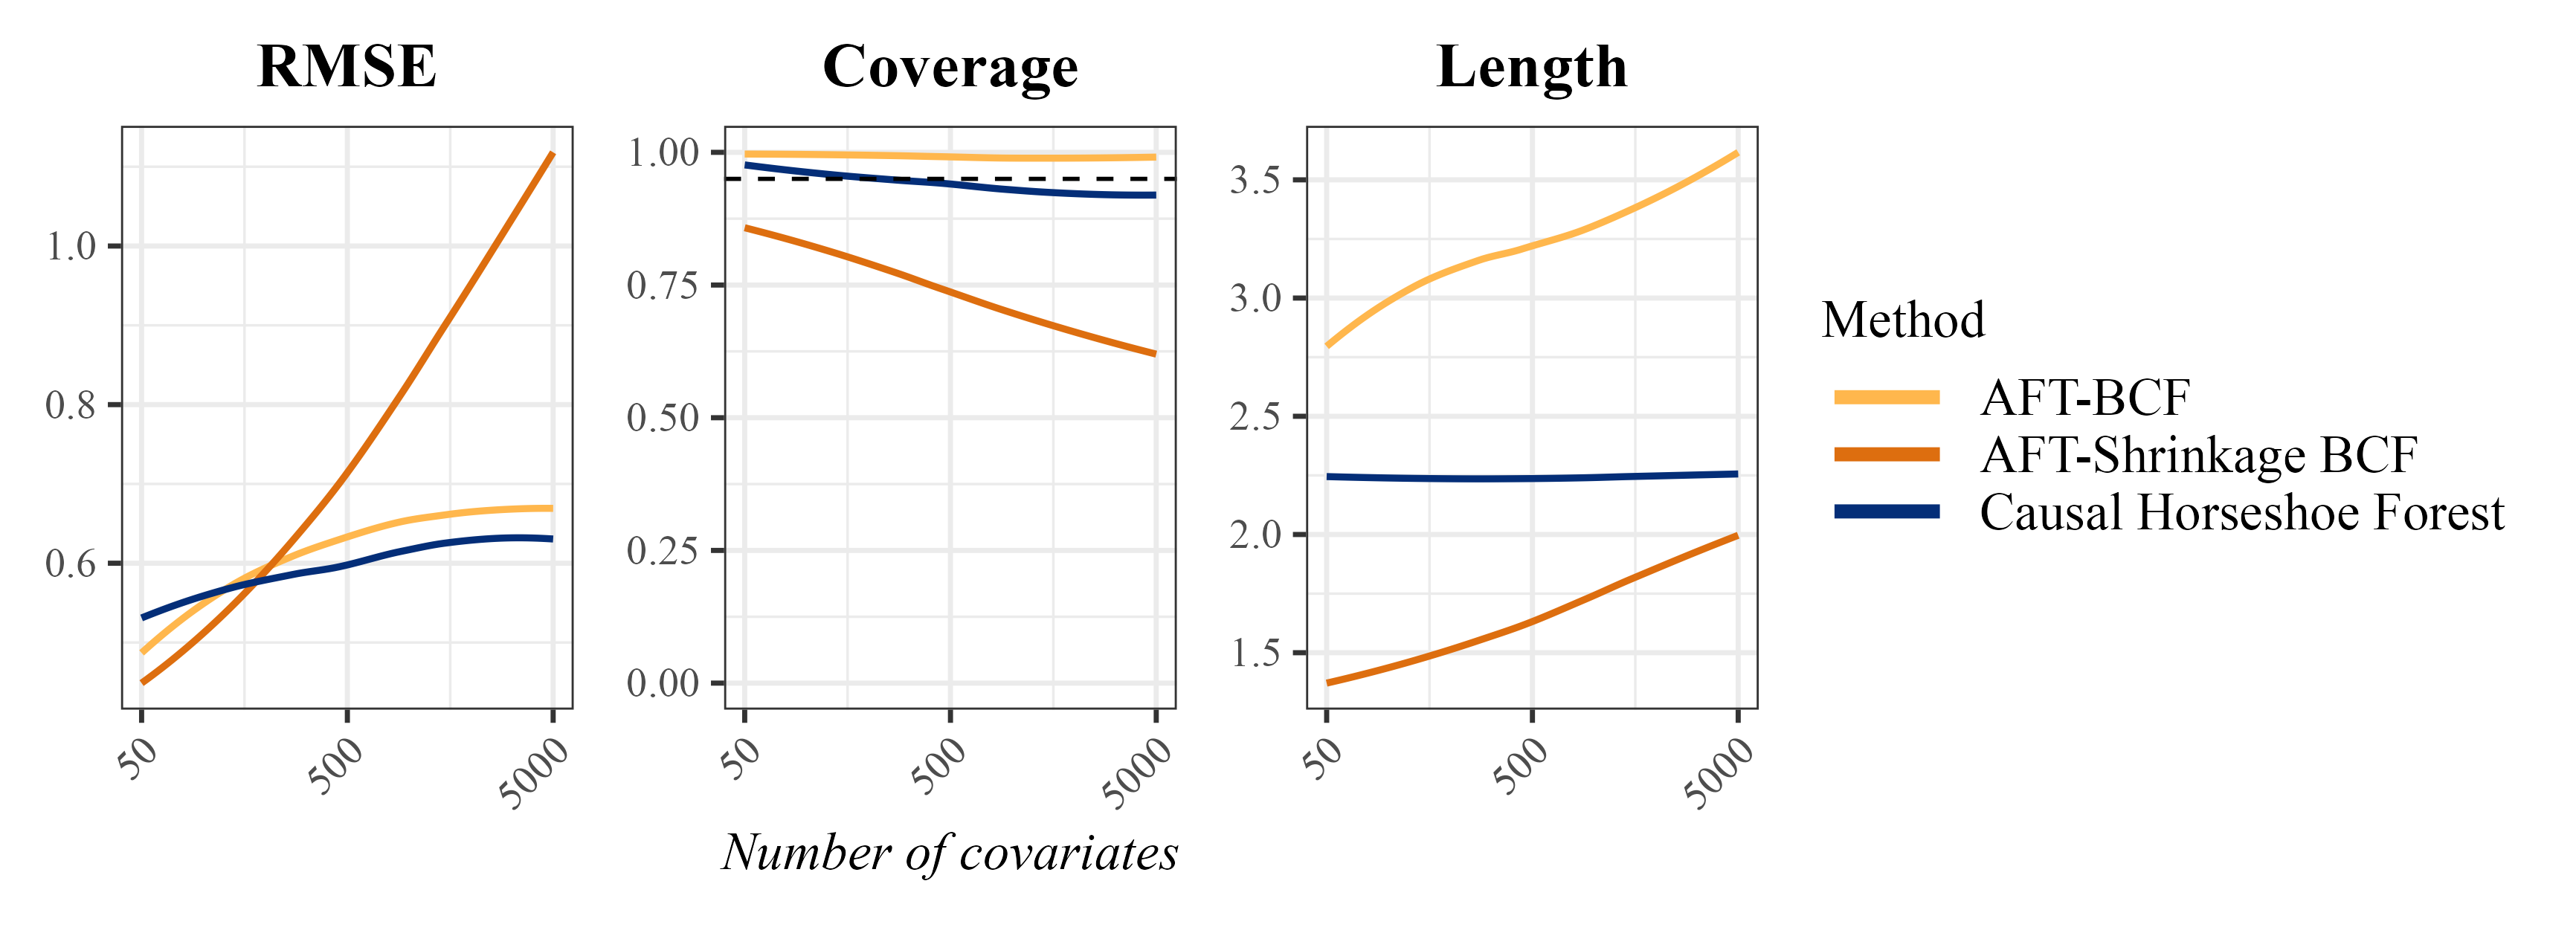
\includegraphics[width=0.95\linewidth]{revision_main_deeper.png}

\smallskip

{\footnotesize Horseshoe Forest: stable RMSE and near-nominal coverage as $p$ grows. AFT-BCF inflates intervals; AFT-Shrinkage BCF loses coverage.}
\end{frame}

%---------------------------------------------------------
\begin{frame}{Simulation 2: regularisation-induced confounding}
\textbf{Setting:} $n = 100$, $p = 500$, censoring $\approx 35\%$.

\bigskip

Two groups of confounders:
\begin{itemize}
  \item $|S| = 5$ \textbf{strong} confounders: strong on both treatment and outcome.
  \item $|W| \in \{1, \ldots, 20\}$ \textbf{weak} confounders: strong on treatment, weak on outcome.
\end{itemize}

\end{frame}

%---------------------------------------------------------
\begin{frame}{Simulation 2: results}
\centering
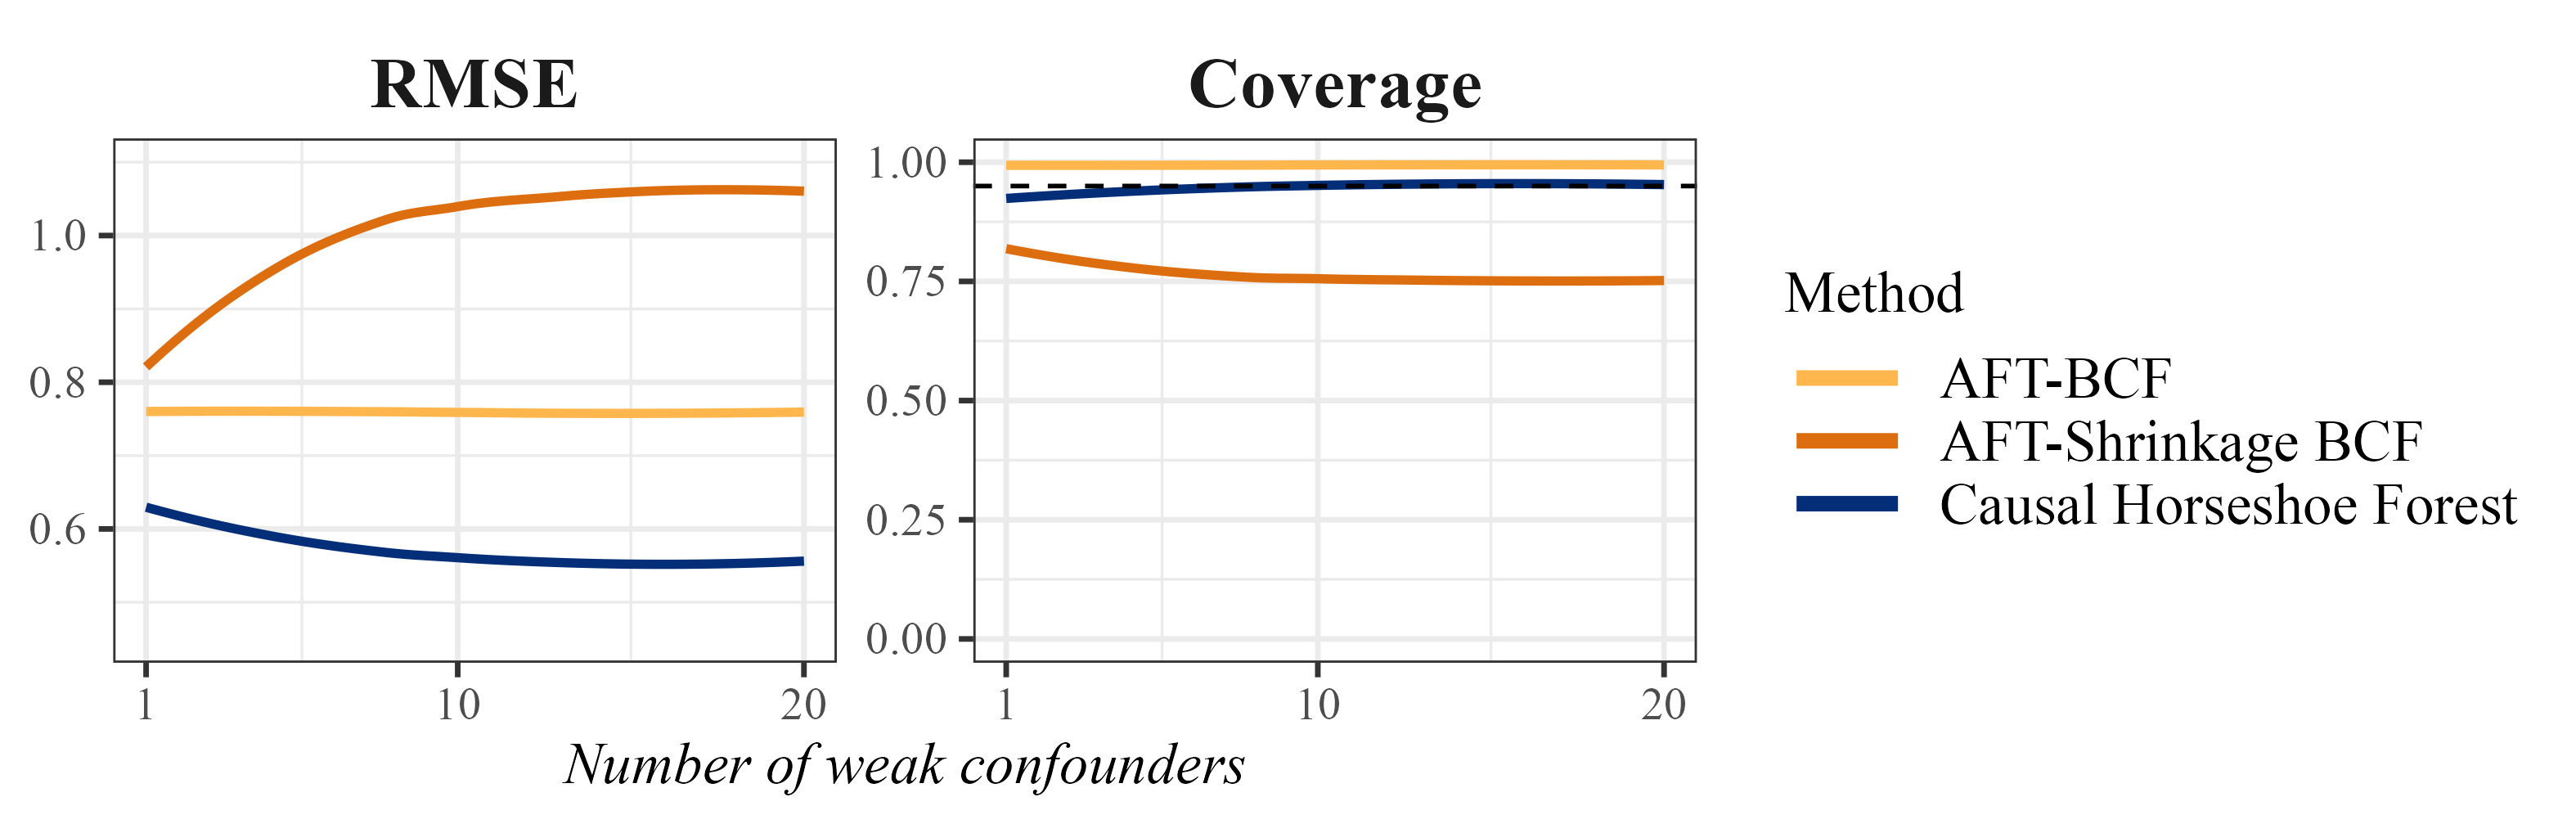
\includegraphics[width=0.95\linewidth]{revision_ric.png}

\smallskip

{\footnotesize Horseshoe Forest stays unbiased as weak confounders accumulate. DART-based competitors drop them and suffer regularisation-induced confounding.}
\end{frame}

%=========================================================
\sectiondivider{Application: pancreatic cancer}
%=========================================================

%---------------------------------------------------------
\begin{frame}{PDAC: the data}
\begin{columns}[T,onlytextwidth]
\begin{column}{0.42\textwidth}
\vspace{0.3cm}
\textbf{TCGA-PAAD cohort:}
\begin{itemize}
  \item $n = 110$ patients (6-month landmark).
  \item 11 clinical covariates $+$ $\sim 3{,}000$ gene expressions.
  \item Censoring $\approx 47\%$.
  \item Median follow-up: 23.3 months.
\end{itemize}

\bigskip

\textbf{Treatment:} adjuvant radiotherapy.
\end{column}
\begin{column}{0.58\textwidth}
\centering
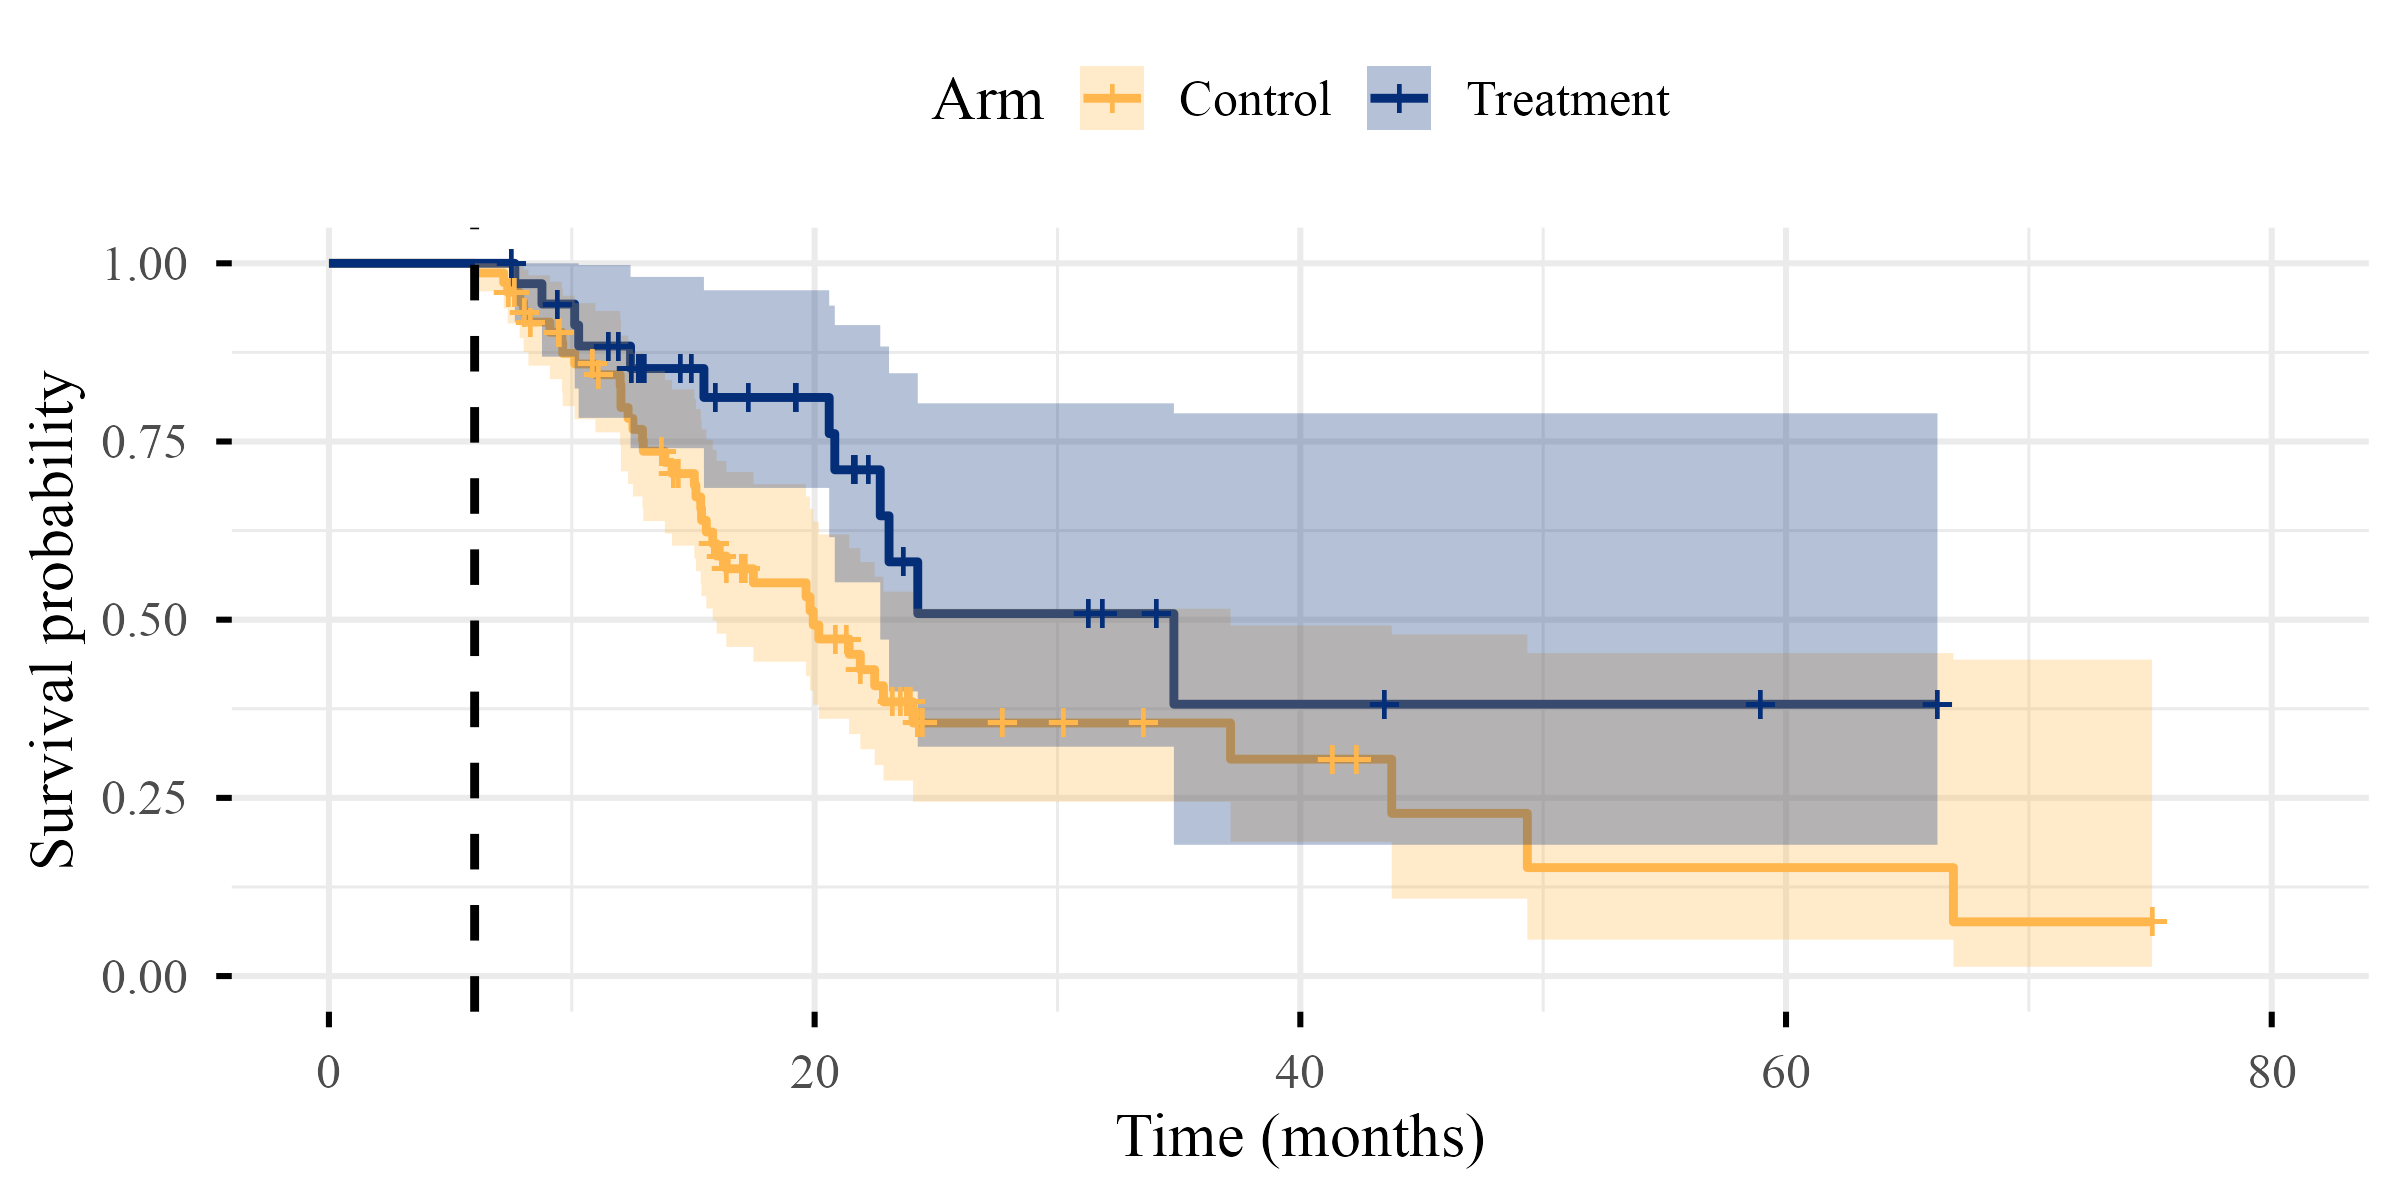
\includegraphics[width=\linewidth]{KM_Landmark.png}
\end{column}
\end{columns}
\end{frame}

%---------------------------------------------------------
\begin{frame}{PDAC: results}
\begin{columns}[c,onlytextwidth]
\begin{column}{0.5\textwidth}
\centering
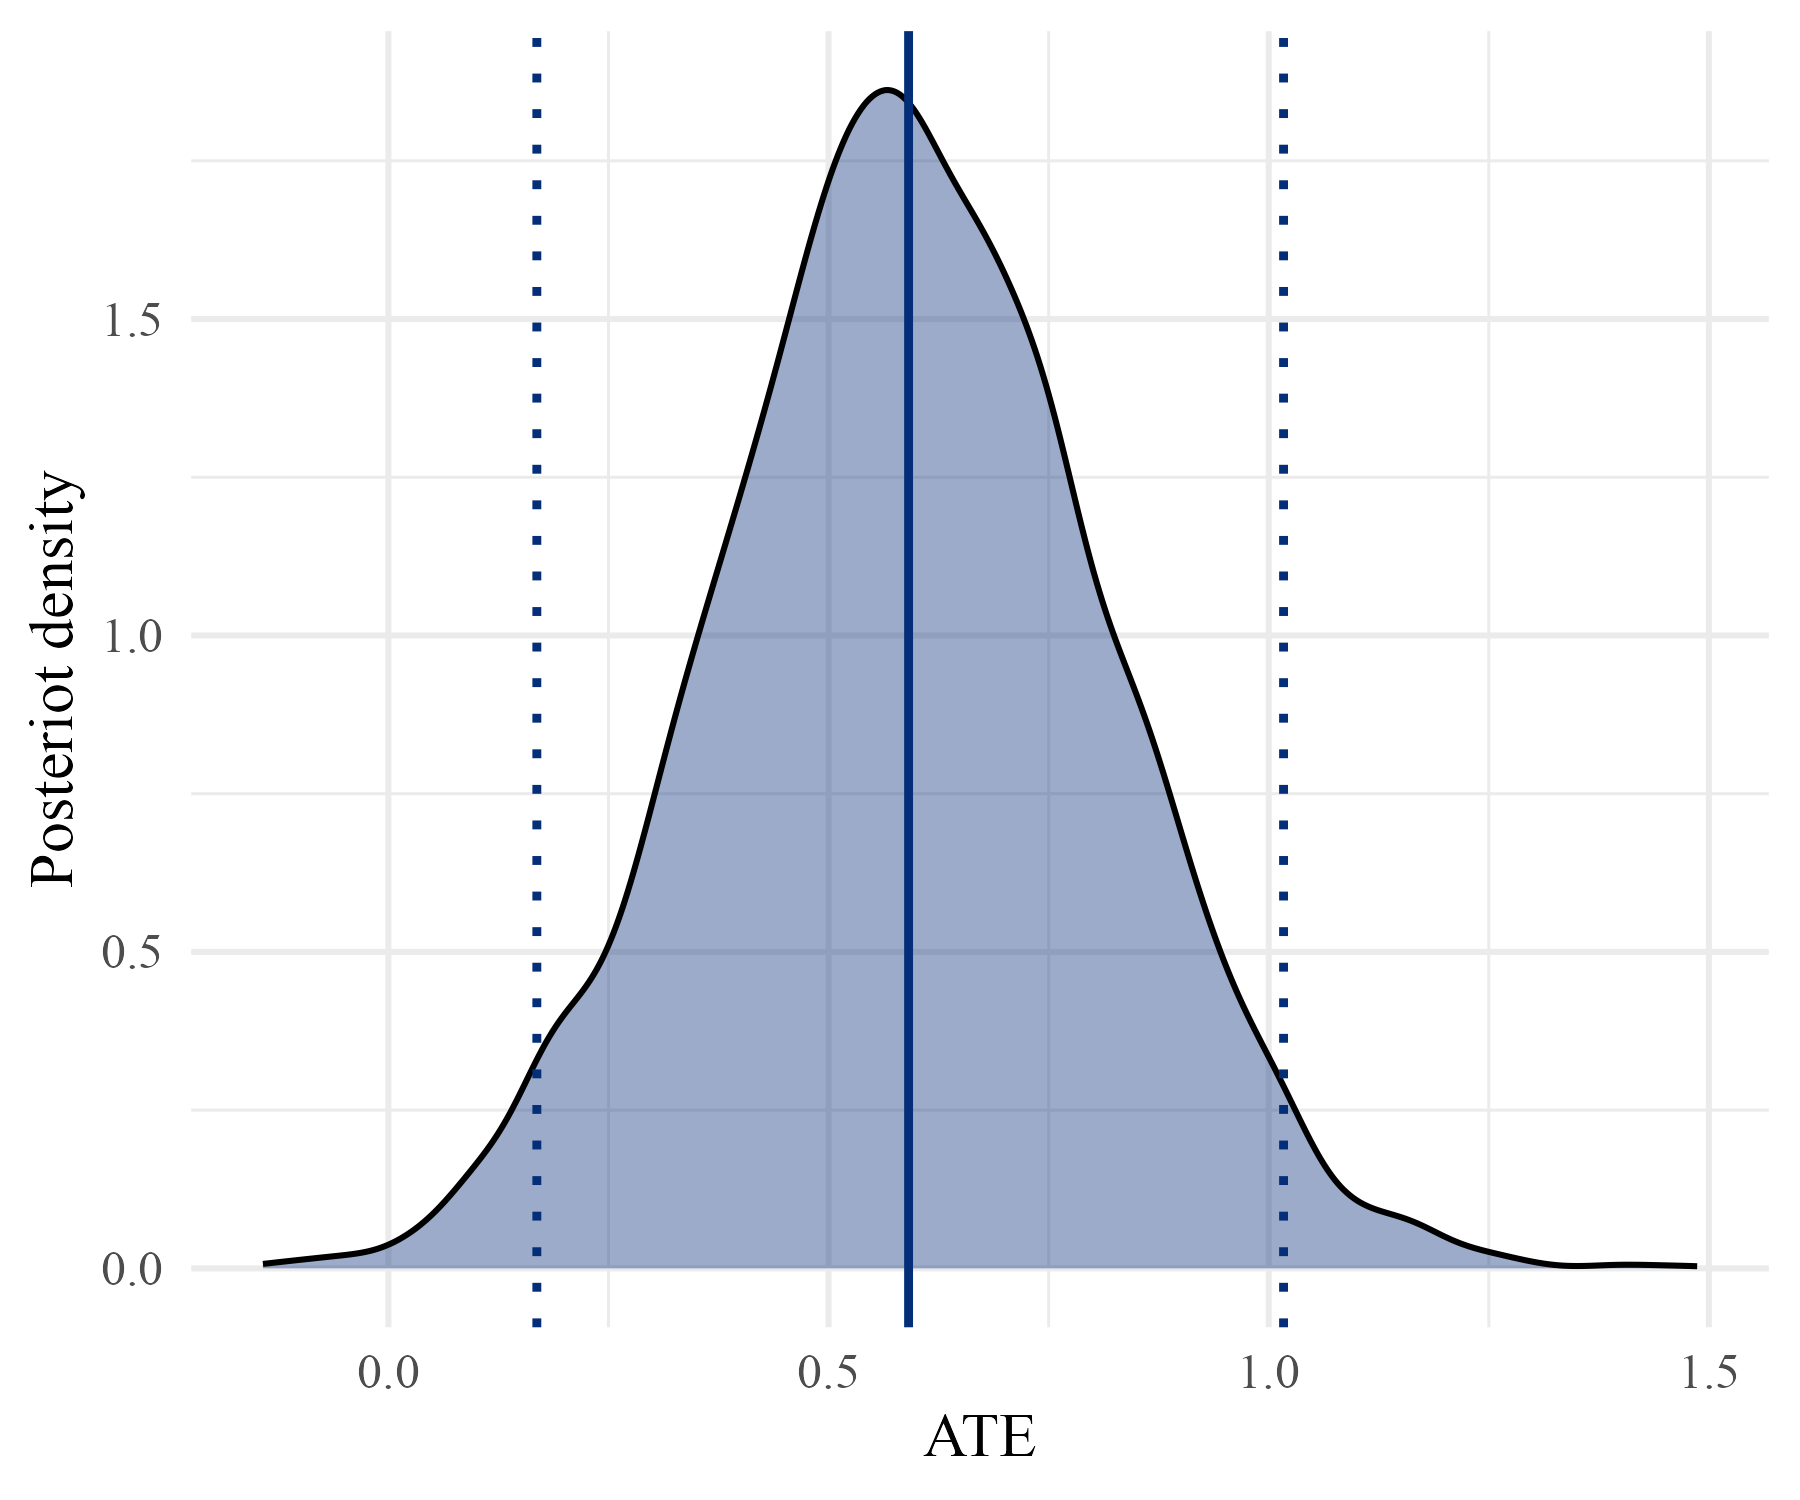
\includegraphics[width=0.9\linewidth]{Plot_posteriorATE_Landmark.png}

\bigskip
{\footnotesize $\widehat{\text{ATE}} \approx 0.55$,\, 95\% CrI $(0.10,\,0.98)$.\\
Acceleration factor $e^{0.55} \approx 1.73$}
\end{column}
\begin{column}{0.5\textwidth}
\centering
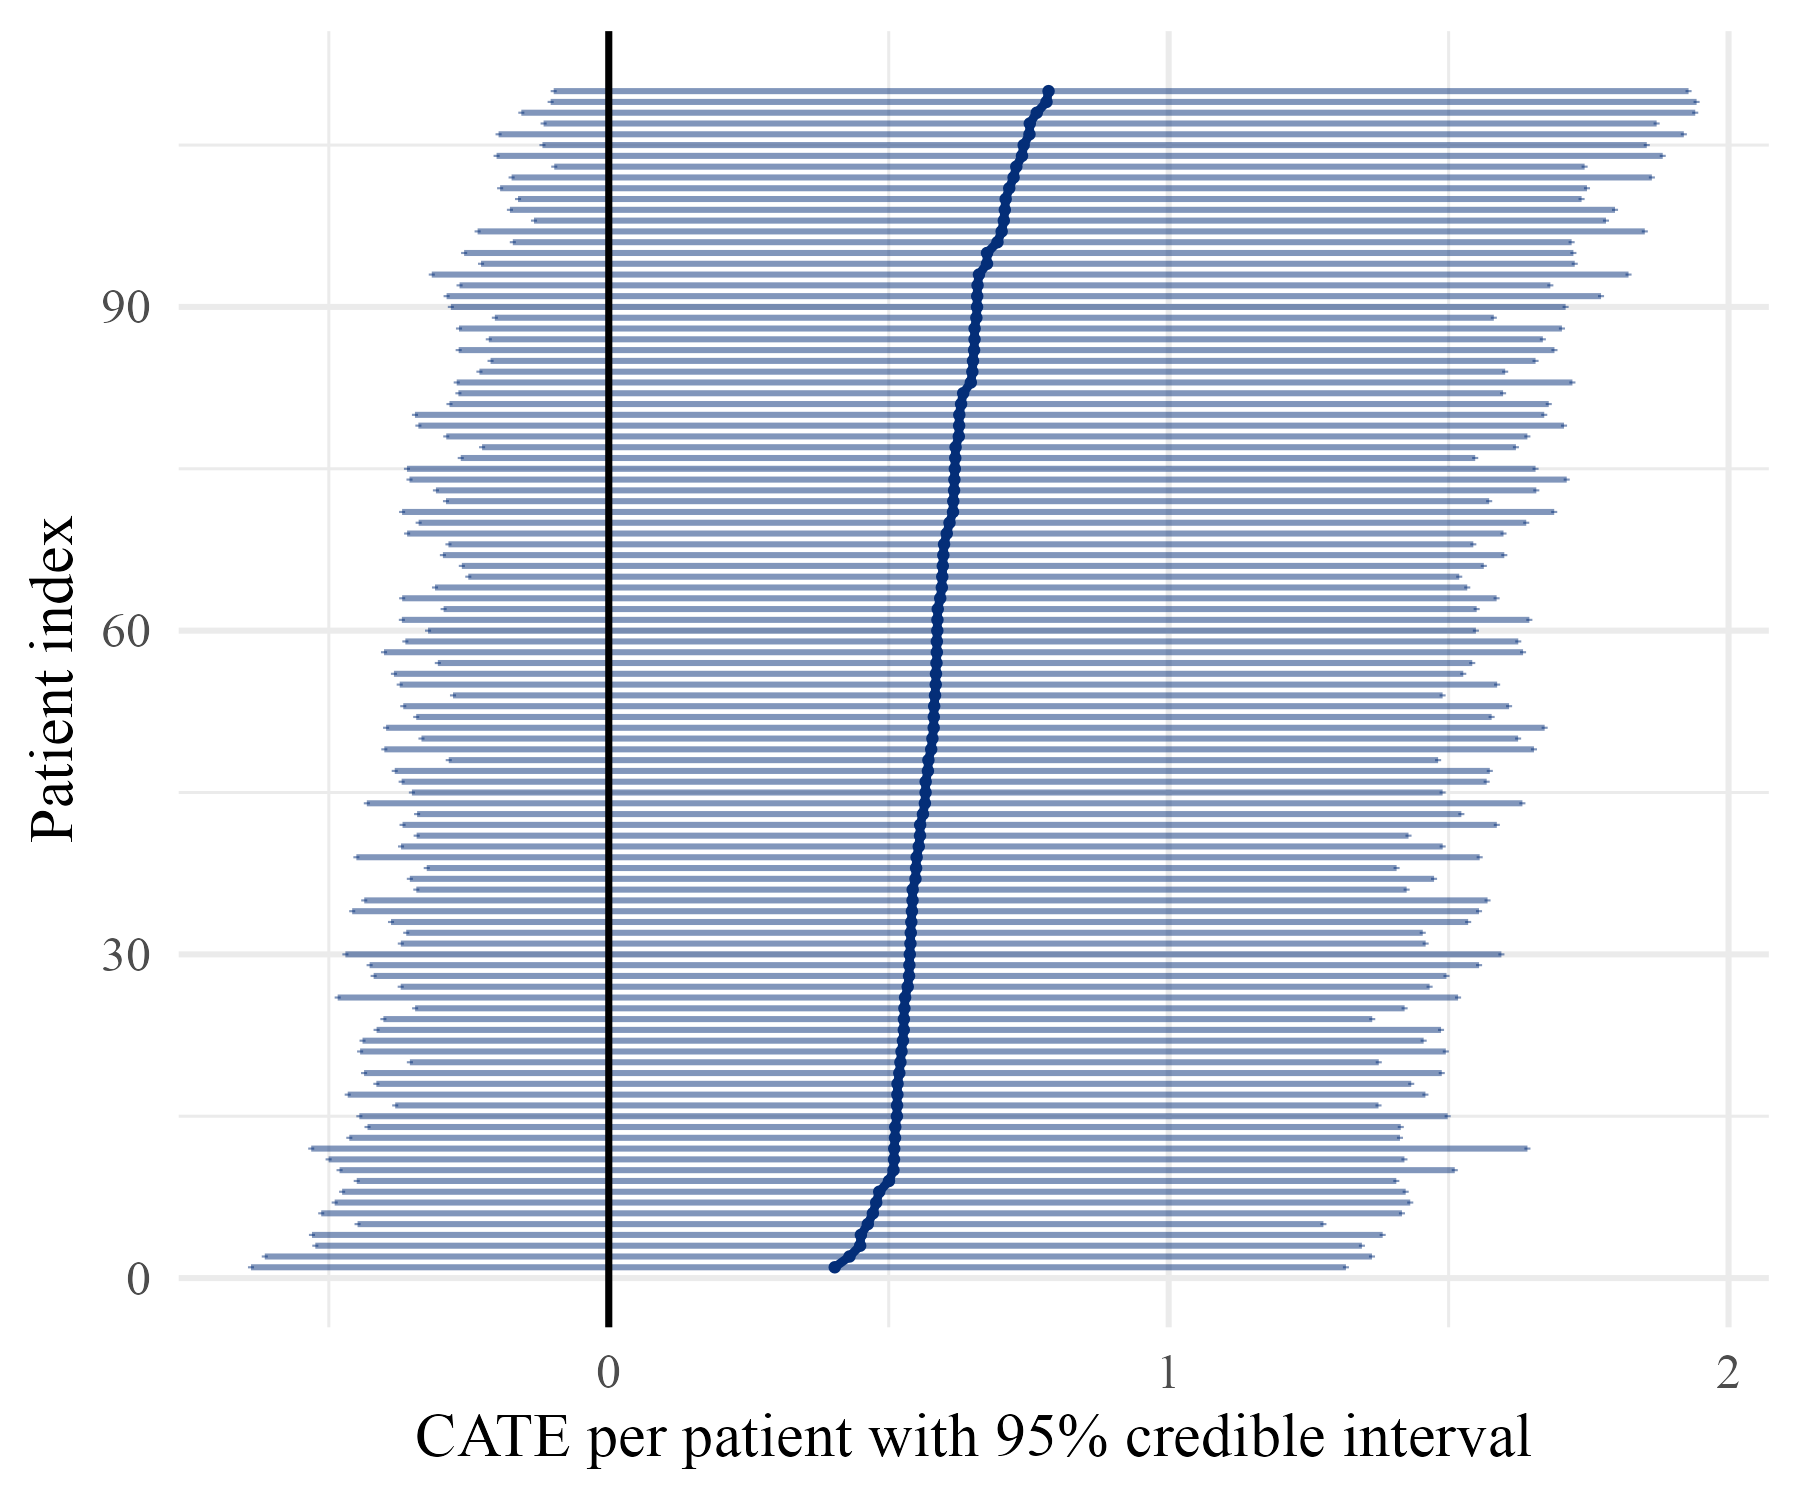
\includegraphics[width=0.9\linewidth]{plot_CATEpatient_Landmark.png}

\bigskip
{\footnotesize \textbf{Predictive performance:} concordance index $= 0.75$.}
\end{column}
\end{columns}
\end{frame}


%---------------------------------------------------------
\begin{frame}{Thanks for your attention!}
\vspace{0.4cm}

\begin{columns}[T,onlytextwidth]

% ---- Left: Paper icon ----
\begin{column}{0.33\textwidth}
\centering
\begin{minipage}[t][2.6cm][c]{\linewidth}\centering

\begin{tikzpicture}[scale=0.95]
\fill[white] (0, 0) rectangle (1.6, 2.2);
\draw[myaccent, thick] (0, 0) rectangle (1.6, 2.2);
\fill[myaccent] (0, 1.85) rectangle (1.6, 2.2);
\draw[white, line width=0.8pt] (0.2, 2.025) -- (1.4, 2.025);
\foreach \y in {1.6, 1.4, 1.2, 1.0, 0.8, 0.6, 0.4} {
  \draw[gray!50, thick] (0.15, \y) -- (1.45, \y);
}
\fill[white] (1.25, 0.4) circle (0.32);
\draw[green!55!black, line width=2pt, line cap=round]
  (1.08, 0.42) -- (1.22, 0.26) -- (1.46, 0.55);
\end{tikzpicture}
\end{minipage}

\bigskip

\begin{minipage}[t][2.0cm][t]{\linewidth}\centering
\textbf{Paper}\\[4pt]
{\footnotesize Accepted at\\ \emph{Bayesian Analysis}.}
\end{minipage}
\end{column}

% ---- Middle: R package hex sticker ----
\begin{column}{0.33\textwidth}
\centering
\begin{minipage}[t][2.6cm][c]{\linewidth}\centering

\includegraphics[height=2.5cm]{ShrinkageTrees_hex.png}
\end{minipage}

\bigskip

\begin{minipage}[t][2.0cm][t]{\linewidth}\centering
\textbf{R package} \texttt{ShrinkageTrees}\\[4pt]
{\footnotesize on CRAN (5000$+$ downloads).\\ Software paper on arXiv soon.}
\end{minipage}
\end{column}

% ---- Right: QR code ----
\begin{column}{0.33\textwidth}
\centering
\begin{minipage}[t][2.6cm][c]{\linewidth}\centering
\qrcode[height=2.5cm]{https://tijn-jacobs.github.io/}
\end{minipage}

\bigskip

\begin{minipage}[t][2.0cm][t]{\linewidth}\centering
\textbf{Stay up to date}\\[4pt]
{\footnotesize \texttt{tijn-jacobs.github.io}}
\end{minipage}
\end{column}

\end{columns}

\vfill

\begin{columns}[c,onlytextwidth]
\begin{column}{0.68\textwidth}
\scriptsize
This work is supported by ERC Grant BayCause, no.\ 101074082. Views and opinions expressed are however those of the author(s) only and do not necessarily reflect those of the European Union or the European Research Council Executive Agency. Neither the European Union nor the granting authority can be held responsible for them.
\end{column}
\begin{column}{0.30\textwidth}
\centering
\includegraphics[width=0.85\linewidth]{"EN-Funded by the EU-POS".jpg}
\end{column}
\end{columns}
\end{frame}

%---------------------------------------------------------
\begin{frame}{References}
\footnotesize
\begin{itemize}
  \item Brathovde, M., Putter, H., Valberg, M., Post, R.A.J.\ (2024). The causal interpretation of acceleration factors. \emph{arXiv:2409.01983}.
  \item Hahn, P.R., Murray, J.S., Carvalho, C.M.\ (2020). Bayesian regression tree models for causal inference: regularization, confounding, and heterogeneous effects. \emph{Bayesian Analysis}, 15(3), 965--1056.
  \item Hougaard, P.\ (1999). Fundamentals of survival data. \emph{Biometrics}, 55(1), 13--22.
  \item Linero, A.R.\ (2018). Bayesian regression trees for high-dimensional prediction and variable selection. \emph{JASA}, 113(522), 626--636.
  \item Zigler, C.M.\ (2016). The central role of Bayes' theorem for joint estimation of causal effects and propensity scores. \emph{The American Statistician}, 70(1), 47--54.
\end{itemize}
\end{frame}

%=========================================================
\appendix
\sectiondivider{Appendix}
%=========================================================

%---------------------------------------------------------
\begin{frame}{Unconfoundedness, intuitively}
\begin{columns}[T,onlytextwidth]
\begin{column}{0.55\textwidth}
\vspace{0.3cm}
\textbf{The worry:} sicker patients may be more (or less) likely to be treated $\Rightarrow$ naive comparison mixes treatment effect with baseline differences.

\bigskip

\textbf{Unconfoundedness:}
\[
T(a) \;\indep\; A \;\big|\; \bm{X}, \qquad a \in \{0,1\}.
\]
\emph{Within each $\bm{X}$, treatment looks as if randomised.}

\bigskip

\alert{Match like-for-like:} same $\bm{X}$ $\Rightarrow$ treatment is the only systematic difference.
\end{column}
\begin{column}{0.40\textwidth}
\centering
\vspace{0.5cm}
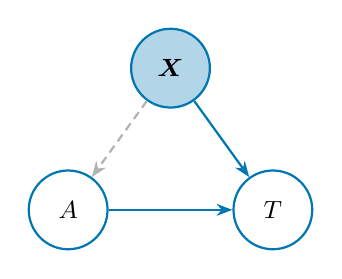
\begin{tikzpicture}[
  every node/.style={circle, draw=myaccent, thick, minimum size=1cm, font=\small},
  arr/.style={-{Stealth[length=2mm]}, thick, myaccent}
]
\node[fill=myaccent!30] (X) at (0,1.4)    {$\bm{X}$};
\node (A) at (-1.3,-0.4) {$A$};
\node (T) at (1.3,-0.4)  {$T$};
\draw[arr, gray!60, densely dashed] (X) -- (A);
\draw[arr] (X) -- (T);
\draw[arr] (A) -- (T);
\end{tikzpicture}

\bigskip
{\footnotesize Conditioning on $\bm{X}$ cuts the dashed back-door arrow.}
\end{column}
\end{columns}
\end{frame}

%---------------------------------------------------------
\begin{frame}{What if we miss a confounder?}
\begin{columns}[T,onlytextwidth]
\begin{column}{0.55\textwidth}
\vspace{0.3cm}
Adjusting for $\bm{X}$ but missing an unmeasured confounder $U$:

\bigskip

\begin{itemize}
  \item Back-door path $A \leftarrow U \rightarrow T$ stays open.
  \item Comparison still picks up the $U$ effect.
  \item \alert{Bias remains --- even with infinite data.}
\end{itemize}

\bigskip

\textbf{High-dimensional consequence:} dropping covariates is risky --- a dropped variable may be a confounder.

\bigskip

\alert{Strategy: keep every covariate in the model.}
\end{column}
\begin{column}{0.40\textwidth}
\centering
\vspace{0.5cm}
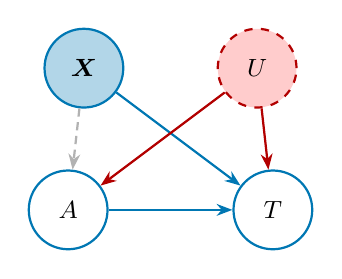
\begin{tikzpicture}[
  every node/.style={circle, draw=myaccent, thick, minimum size=1cm, font=\small},
  arr/.style={-{Stealth[length=2mm]}, thick, myaccent}
]
\node[fill=myaccent!30] (X) at (-1.1,1.4)  {$\bm{X}$};
\node[draw=red!70!black, fill=red!20, dashed] (U) at (1.1,1.4)   {$U$};
\node (A) at (-1.3,-0.4) {$A$};
\node (T) at (1.3,-0.4)  {$T$};
\draw[arr, gray!60, densely dashed] (X) -- (A);
\draw[arr] (X) -- (T);
\draw[-{Stealth[length=2mm]}, thick, red!70!black] (U) -- (A);
\draw[-{Stealth[length=2mm]}, thick, red!70!black] (U) -- (T);
\draw[arr] (A) -- (T);
\end{tikzpicture}

\bigskip
{\footnotesize Unmeasured $U$ leaves an open back-door path $A \leftarrow U \rightarrow T$.}
\end{column}
\end{columns}
\end{frame}

\end{document}
